\chapter{RUMIS - Nonmonotonic Rule Mining System}\label{chap:system}

RUMIS stands for Nonmonotonic Rule Mining System which is the main tool developed in the current work. This chapter describes in details the practical implementation of theory framework presented in Chapter~\ref{chap:frame} and uses background definitions in Chapter~\ref{chap:back}. Organization of the chapter is as follows, first, an overview of the RUMIS is discussed. Second, the implementations of main components in the system are presented. Finally, we talk about installation and usage of the system.

\section{System Overview}
\label{sec:overview}

There are six components in RUMIS as presented in Figure~\ref{system_overview} with arrows indicating the data flow from input to output. RUMIS mines the nonmonotonic rules from the original graph in the following steps:

\begin{itemize}
\item In (1), a KG $\cG$ as an input is passed to RUMIS. It is then stored and indexed into the system by Component 1~\ref{data_indexing} which is exploited to speed up computation in the next steps.
\item In (2), Horn rules are mined by Component 2 from facts indexed into RUMIS.
\item In (3), normal and abnormal sets are found by Component 3 based on KG $\cG$ and mined Horn rules in the previous step.
\item With normal and abnormal sets known for each Horn rule, (4) represents for finding exception witness sets in Component 4.
\item In (5) and (6), exception candidates are ranked in Component 6 using a measure plugged by Component 5. RUMIS allocates a separate component for measure plugin to flexibly extend ranking criteria in the future.
\item In (7), after being ranked, the best revision for each Horn rule is added to the output of RUMIS.
\end{itemize}

\begin{figure}[ht]
\centering
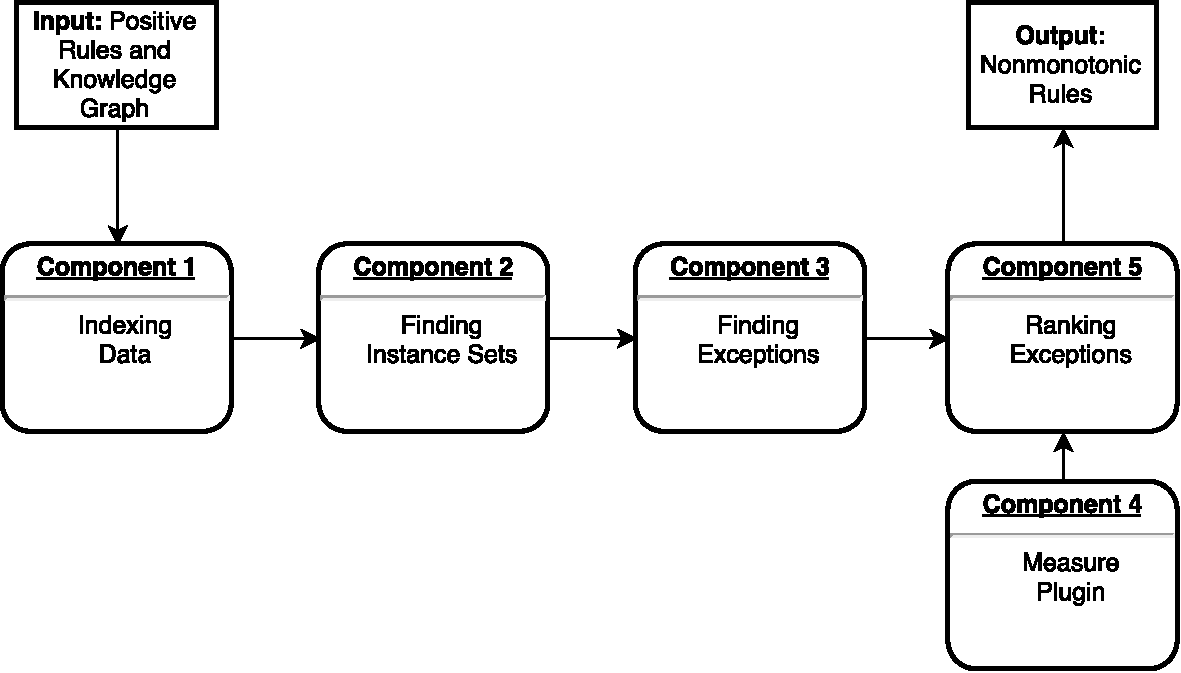
\includegraphics[width=0.85\textwidth]{figures/system_overview}
\caption{Components of RUMIS}
\label{system_overview}
\end{figure}

\section{Implementation}

In this section, the main components mentioned in Section~\ref{sec:overview} are described in details. To simplify the problem of \textit{language bias}, the implementation of RUMIS only takes the following positive rule form into consideration:

\begin{equation}
r2: h(X, Z) \leftarrow p(X, Y), q(Y, Z)
\label{form2}
\end{equation}

Where $h$, $p$, $q$ are binary predicates from KG $\cG$, these notations and the form~\ref{form2} ($r2$) are used in the rest of this thesis.

\subsection{Data Indexing}
\label{data_indexing}

\begin{figure}[ht]
\centering
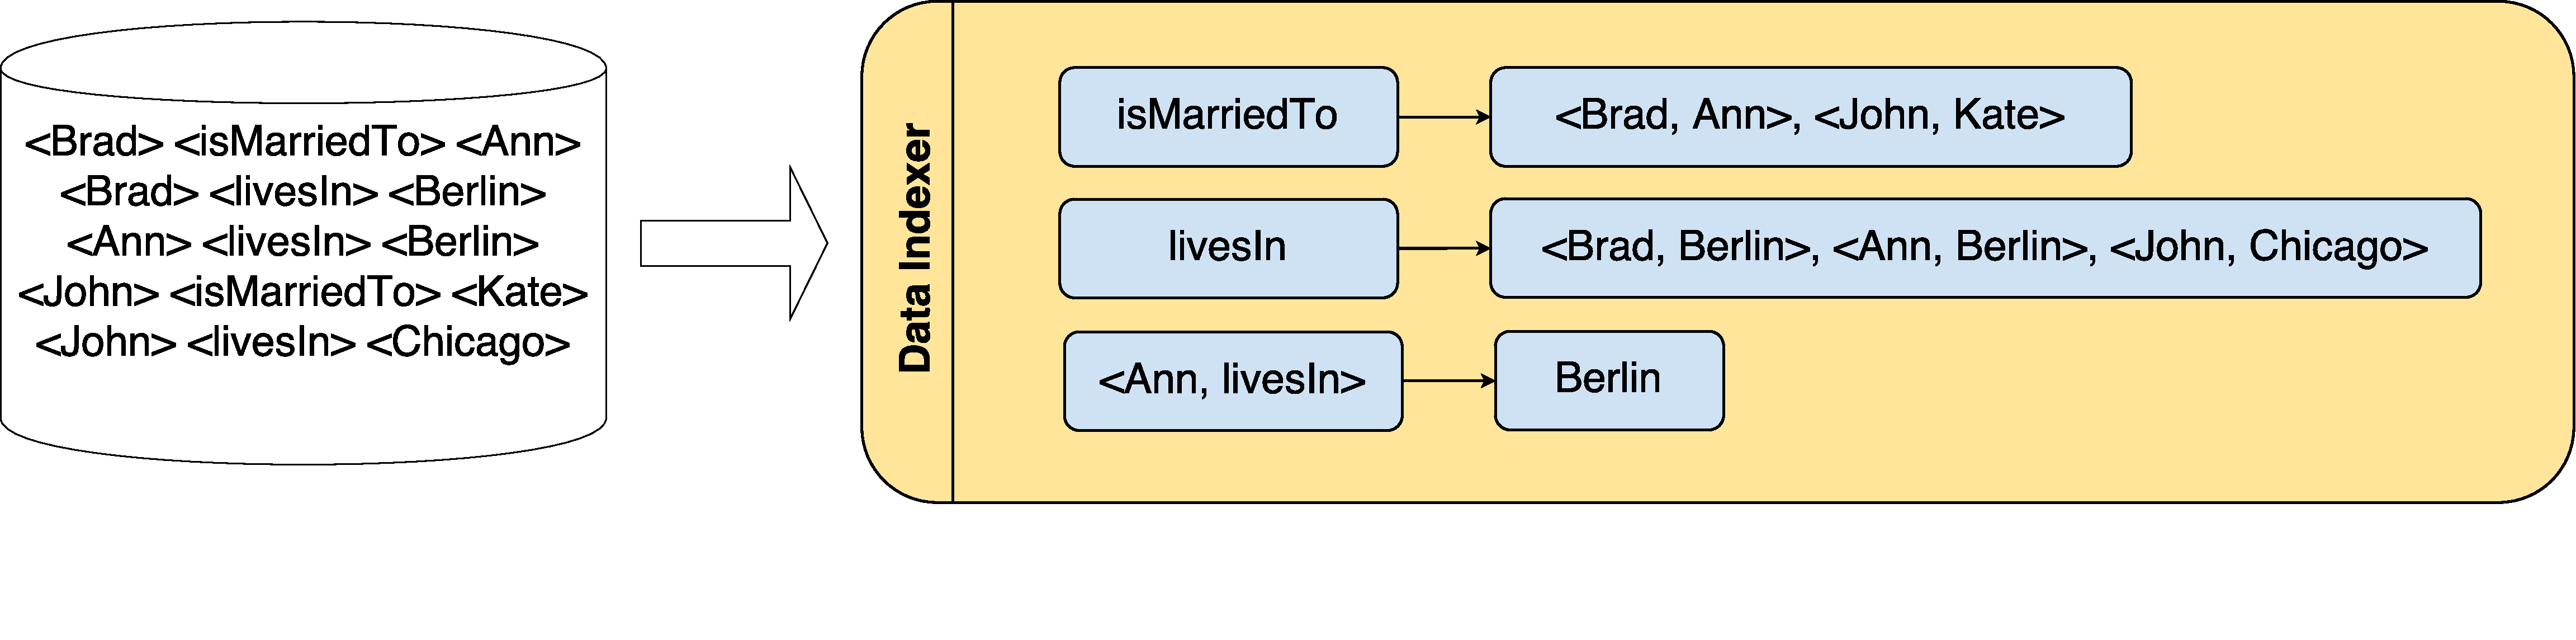
\includegraphics[width=1.0\textwidth]{figures/data_indexing}
\caption{RUMIS Data Indexer}
\label{data_indexing}
\end{figure}

Since the KG $\cG$ can be huge, it takes a long time to find (ab)normal instances and exception witness sets of a positive rule. To overcome this, data indexing is taken into consideration to speed up processing data. In a traditional search engine, terms such as words, n-grams are indexed into the system and their corresponding posting lists are a collection of documents containing them. The same intuition can be applied to relational setting in the current work. Indeed, RUMIS treats every fact as a document and the terms can be subjects, predicates, objects or some combinations of them.

To be specific, Figure~\ref{data_indexing} illustrates data indexed from part of KG in Figure~\ref{fig1.1}. In the figure, based on the index, if predicate \textit{isMarriedTo} is given, we can find set of subject-object pairs corresponding to this relation, i.e., \textit{$<$Brad, Ann$>$} and \textit{$<$John, Kate$>$}. Besides, objects can be found if we have at hand their corresponding subjects and relations. For example, we can get ``Berlin" as an answer to the question: ``Where does Ann live" based on data indexing illustrated in the Figure~\ref{data_indexing}. In this example, the term is the combination of subjects and predicates. More formally, Data Indexing provides the following functions that are exploited in the rest components:

\begin{itemize}
\item \textit{getPredicateSubjectSet($\cG$, object):} This function returns a set of predicate-subject pairs corresponding to a given \textit{object} in KG $\cG$.
\item \textit{getPredicateSet($\cG$, subject, object):} A set of predicates corresponding to input \textit{subject, object} entities are found in this function.
\item \textit{getSubjectSet($\cG$, predicate, object):} A set of subjects are an output for given \textit{predicate, object} based on this function.
\item \textit{getSubjectObjectSet($\cG$, predicate):} This function is to find a set of subject-object pairs if we have \textit{predicate} at hand as a parameter.
\end{itemize}

\subsection{Positive Rule Mining}

Positive Rule Mining finds Horn rule $r2$ in the form~\ref{form2} with high \textit{absolute support}. The way how this works is illustrated in Algorithm~\ref{algo1} with the following steps. First, in line 1, \textit{absSupp} is created with the aim to store absolute support of positive rules. More specifically, $absSupp[hpq]$ is the absolute support of rule \textit{r2}. Second, for each triple \textit{$<$Y q Z$>$} from KG $\cG$, a set of pairs \textit{X, p} are found such that \textit{X p Y} is in $\cG$ (line 2 and 3). Command in line 3 is executed using \textit{getPredicateSubjectSet} function in Data Indexing component. Third, from line 5 to 6, with \textit{X, Z} found in the previous step, RUMIS searches for every relation $h$ s.t. \textit{$<$X h Z$>$} is in $\cG$. At this point, it is guaranteed that \textit{h(X, Z), p(X, Y), q(Y, Z)} holds true. After that, in line 7, absolute support of the rule \textit{r2} is increased by $1$. Finally, all rules are sorted in decreasing order of absolute support.

\IncMargin{1.5em}
\begin{algorithm}[H]
\DontPrintSemicolon
\SetAlgoLined
\SetKwInOut{Input}{Input}\SetKwInOut{Output}{Output}
\Input{KG $\cG$}
\Output{Set of positive rules with the same form as $r2$}
\BlankLine
$absSupp \leftarrow \{\}$\\
\BlankLine
\ForEach{Triple $YqZ$ in $\cG$} {
    \BlankLine
	$pXSet \leftarrow getPredicateSubjectSet(\cG, Y)$\\
	\ForEach{Pair $pX$ in $pXSet$} {
		$hSet \leftarrow getPredicateSet(\cG, X, Z)$\\
		\ForEach{Predicate $h$ in $hSet$} {
			$absSupp[hpq]++$\\
		}
	}
}
\BlankLine
Sort $hpq$ according to deacreasing order of $absSupp[hpq]$\\
\Return $absSupp$\\
\caption{Positive Rule Mining}
\label{algo1}
\end{algorithm}
\DecMargin{1.5em}

\subsection{Normal and Abnormal Set Mining}

This component explores normal and abnormal sets of rule \textit{r2} in Algorithm~\ref{algo2} as follows. First, in lines 1 and 2, (ab)normal sets are created. Second, for each pair \textit{Y, Z} s.t. \textit{$<$Y q Z$>$} is in $\cG$, a set of $X$ in the fact \textit{$<$X p Y$>$} from the KG are found based on Data Indexing component (line 3 to 5). At this point, it is guaranteed that \textit{X, Y, Z}  fulfills the body of rule \textit{r2}. Finally, for every $X$ found in the previous step, \textit{$<$X h Z$>$} is verified to be in the the KG or not. If it is in $\cG$, \textit{$<$X Z$>$} is added to the normal set, otherwise it is added to the abnormal set.

\IncMargin{1.5em}
\begin{algorithm}[H]
\DontPrintSemicolon
\SetAlgoLined
\SetKwInOut{Input}{Input}\SetKwInOut{Output}{Output}
\Input{KG $\cG$, $h$, $p$, $q$ predicates in the rule $r2$}
\Output{Normal and abnormal sets of the rule $r2$}
\BlankLine
$NS \leftarrow \{\}$\\
$ABS \leftarrow \{\}$\\
$YZSet \leftarrow getSubjectObjectSet(\cG, q)$\\
\BlankLine
\ForEach{Pair $YZ$ in $YZSet$} {
    \BlankLine
	$XSet \leftarrow getSubjectSet(\cG, p, Y)$\\
	\ForEach{$X$ in $XSet$} {
	\uIf{$XhZ$ is in $\cG$} {
		Add $XZ$ to $NS$\\
	}
	\uElse {
		Add $XZ$ to $ABS$\\
	}
	}
}
\BlankLine
\Return $NS$ and $ABS$\\
\caption{Normal and Abnormal Set Mining}
\label{algo2}
\end{algorithm}
\DecMargin{1.5em}

\subsection{Exception Witness Set Mining}

Binary predicate exception candidates of positive rules \textit{r2} are an output for Algorithm~\ref{algo3}. More specifically, our goal is to find exceptions with the form \textit{e(X, Z)}, they are then inserted to the body of $r2$ to get its revised rule \textit{h(X, Z) :- p(X, Y), q(Y, Z), not e(X, Z)}. Similarly, unary exceptions \textit{e(X)} or \textit{e(Z)} can be mined in an equivalent way with binary ones. As regards Algorithm~\ref{algo3}, there are several steps as follows, first, normal and abnormal instance sets are found from Algorithm~\ref{algo2} in line 1 and 2. In addition, $EWS+$ and $EWS-$ (i.e., set of relations between \textit{$<$X Z$>$} in the abnormal and normal sets, resp.) are created (line 3 and 4). Second, for every pair \textit{$<$X Z$>$} in the abnormal set, all relations between them are added to the $EWS+$ (line 5 to 8). After that, similar stage is applied for $EWS-$ from line 9 to 12. Finally, exception witness set $EWS$ is calculated as the difference between $EWS+$ and $EWS-$.

\IncMargin{1.5em}
\begin{algorithm}[H]
\DontPrintSemicolon
\SetAlgoLined
\SetKwInOut{Input}{Input}\SetKwInOut{Output}{Output}
\Input{KG $\cG$, $h$, $p$, $q$ predicates of the rule $r2$}
\Output{Exception witness set of the rule $r2$}
\BlankLine
$NS \leftarrow getNormalSet(\cG, h, p, q)$\\
$ABS \leftarrow getAbnormalSet(\cG, h, p, q)$\\
$EWS+ \leftarrow \{\}$\\
$EWS- \leftarrow \{\}$\\
\BlankLine
\ForEach{Pair $XZ$ in $ABS$} {
	$pSet \leftarrow getPredicateSet(\cG, X, Z)$\\
	$EWS+$ $\leftarrow$ $EWS+$ $\cup$ $pSet$\\
}
\ForEach{Pair $XZ$ in $NS$} {
	$pSet \leftarrow getPredicateSet(\cG, X, Z)$\\
	$EWS-$ $\leftarrow$ $EWS-$ $\cup$ $pSet$\\
}
$EWS$ $\leftarrow$ $EWS+$ $\setminus$ $EWS-$\\
\Return $EWS$\\
\caption{Exception Witness Set Mining}
\label{algo3}
\end{algorithm}
\DecMargin{1.5em}

\subsection{Measure Plugin}

To be easy to plugin and test another rule quality criteria, the measure plugin is designed as a separate component. There are two main measures in the current implementation: confidence and conviction. While the former is a good choice for descriptive purpose, its predictive quality is not as good as that of the latter~\cite{ref46}. Since the main concern of this thesis is to revise Horn rules and subsequently predict accurate facts to expand the original KG, conviction is the main measure in RUMIS.

\subsection{Exception Ranking}

Figure~\ref{pm_ranking} shows some arrows representing for the communications between different parts in (O)PM ranking. In general, the communications express the intuition for the ranking as follows.

\begin{itemize}
\item From a KG $\cG$ and a set of Horn rules, EWS mining is executed to find exception candidates for each Horn rule in (1).
\item (2) shows that some rules with exceptions (revisions) are used to infer new facts from the original KG. The strategy how to select the revisions is the difference between PM and OPM ranking.
\item $\cG'$, i.e., original KG $\cG$ with new predicted facts, is exploited to rank exceptions for each Horn rule in (3). The combination of steps (2) and (3) describes the interaction of different rules, i.e, facts generated by other revisions are taken into account to measure quality of a particular nonmonotonic rule. That is also the intuition of (O)PM ranking.
\item (4) is a process that exceptions are ranked by Component 5, the best exception is chosen to be added in final revision set.
\end{itemize}

\begin{figure}[ht]
\centering
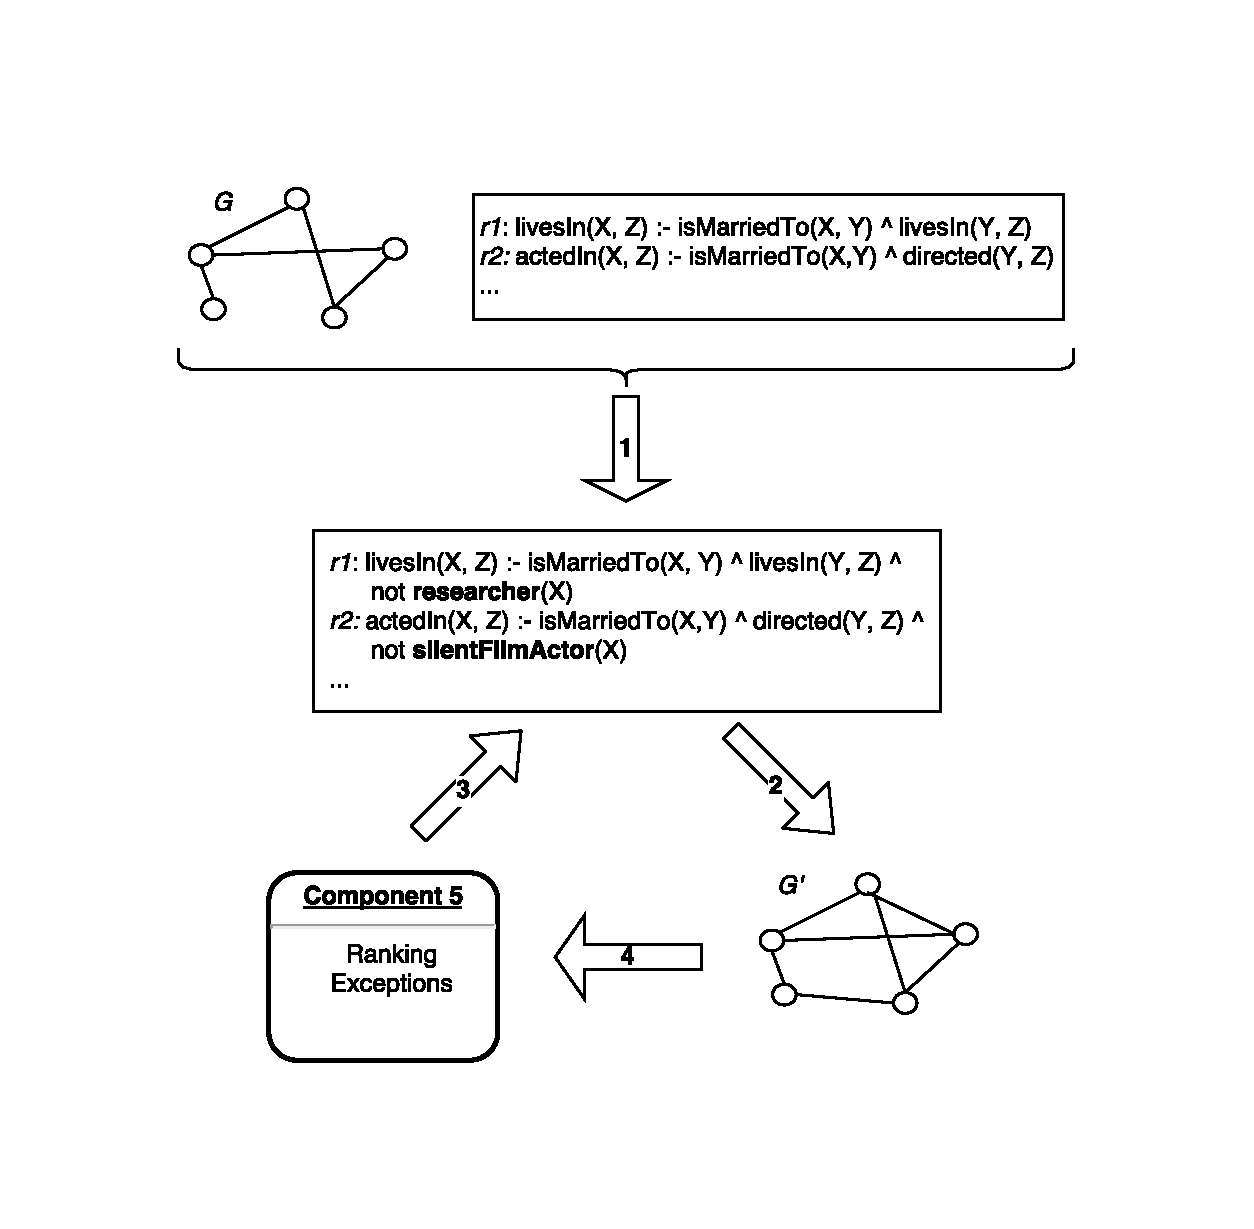
\includegraphics[width=1.0\textwidth]{figures/ranking}
\caption{(Ordered) Partial Materialization Ranking}
\label{pm_ranking}
\end{figure}

\textbf{PM Ranking.} This function is executed in the Algorithm~\ref{pm_ranking_algo} with the following steps. In lines 1 and 2 of the algorithm, we clone an original graph $\cG$ to $\cG'$ and create empty nonmonotonic rule set $R_NM$. After that, from line 3 to 5, for every Horn rule $r$ in $R_H$, all new facts produced by $r$ and not by any revision of $r$ from $\cG$ (safely predicted facts of $r$ [should be defined in background section]) are added to $\cG'$ using Data Indexing component. In other words, all exceptions of $r$ are used to reduce the possibility of wrongly predicted facts. Besides, RUMIS is conservative in producing new facts since the system applies revisions to $\cG$ instead of $\cG'$ in every iteration. This eliminates the cases that wrong facts introduce many incorrect ones in the future process. 

Now RUMIS is ready for PM ranking strategy, in line 7, for each Horn rule $r$, indexes of its safely predicted facts are removed from $\cG'$. This step is to make sure that safely predicted facts of all other rules ($r$ excluded) are exploited to determine quality of $r$ (line 8). Thanks to this, the interaction between nonmonotonic rules are taken into consideration for the ranking. After that, the best revision of $r$ is added to the final result in line 9. Line 10 shows a step that undoes what is done in line 7, i.e., safely predicted facts of rule $r$ based on $\cG$ is added to $\cG'$ again. This guarantees the same setting in the next iteration can be processed with a new rule.

\IncMargin{1.5em}
\begin{algorithm}[H]
\DontPrintSemicolon
\SetAlgoLined
\SetKwInOut{Input}{Input}\SetKwInOut{Output}{Output}
\Input{KG $\cG$, set of positive rules $\cR_{H}$}
\Output{Set of best revisions $R_{NM}$ for the given positive rules $R_H$}
\BlankLine
$\cG' \leftarrow \cG$\\
$R_{NM} \leftarrow \{\}$\\
\BlankLine
\ForEach{Rule $r$ in $R_H$} {
	Generate safely predicted facts of $r$ w.r.t. $\cG$ then index these facts to $\cG'$\\
}
\BlankLine
\ForEach{Rule $r$ in $R_H$} {
	Generate safely predicted facts of $r$ w.r.t. $\cG$ then remove these facts' indexes from $\cG'$\\
	Rank exceptions of $r$ based on $\cG'$, choose $r'$ as the best revision of $r$\\
	Add $r'$ to $R_{NM}$\\
	Generate safely predicted facts of $r$ w.r.t. $\cG$ then index these facts to $\cG'$ (undoes step in line 7)\\
}
\Return $R_{NM}$\\
\caption{PM Ranking}
\label{pm_ranking_algo}
\end{algorithm}
\DecMargin{1.5em}

\textbf{OPM Ranking.} This function (Algorithm~\ref{opm_ranking_algo}) is similar to PM ranking, the only difference is the way how to select revisions to expand KG $\cG'$. In details, there are several steps in the algorithm as follows. From line 1 to 2, the process is executed in the same way as in PM ranking. All the Horn rules are then sorted in decreasing order of conviction measure (line 3). Similar to PM, for each Horn rule $r$ in $R_H$ (line 4), OPM ranking chooses the best revision of $r$ based on $G'$ for the final result (line 5 and 6). After that, in line 7, safely new facts are predicted to update KG $\cG'$.

Intuitively, all safely predicted facts from previous rules w.r.t. $\cG$ are added to $\cG'$ which is exploited to assess quality of $r$. In OPM ranking, the order of Horn rules regarding the conviction matters, i.e., the higher conviction quality of an Horn rule, the more important impact it plays on the other rules. In other words, OPM is more conservative than PM ranking, only safely predicted facts of better Horn rules may be taken into account to revise a particular one.

\IncMargin{1.5em}
\begin{algorithm}[H]
\DontPrintSemicolon
\SetAlgoLined
\SetKwInOut{Input}{Input}\SetKwInOut{Output}{Output}
\Input{KG $\cG$, set of positive rules $\cR_{H}$}
\Output{Set of best revisions $R_{NM}$ for the given positive rules $R_H$}
\BlankLine
$\cG' \leftarrow \cG$\\
$R_{NM} \leftarrow \{\}$\\
Sort all rules in $R_H$ according to the decreasing order of conviction\\
\BlankLine
\ForEach{Rule $r$ in $R_H$} {
	Rank exceptions of $r$ based on $\cG'$, choose $r'$ as the best revision of $r$\\
	Add $r'$ to $R_{NM}$\\
	Generate safely predicted facts of $r$ w.r.t. $\cG$ then index these facts to $\cG'$\\
}
\Return $R_{NM}$\\
\caption{OPM Ranking}
\label{opm_ranking_algo}
\end{algorithm}
\DecMargin{1.5em}

\section{Usage}

[ToDo: Describe installation and usage]
